\ifgerman{\chapter{Evaluierung}}{\chapter{Evaluation}}
\label{ch:evaluation}

Evaluating a classification algorithm also known as classification model is necessary to find how competent the algorithm is on data it has never seen. The classification model generates probabilities when given the of predicting on unobserved data. 

\section{Experimental Setup}
Most of the experiments were carried out on \textit{Google Colab} is a free google service that provides Jupyter notebooks with Python environment that stores the notebooks on Google Drive. It provides a GPU (Graphics Processing Unit) or TPU (Tensor Processing Unit) and has pre-installed various popular machine learning and deep learning framework. The exact detail of the system is listed in the \ref{table:HWsetup}

\begin{table}[!ht]
\centering
\begin{tabular}{cc}
\hline
\textbf{Hardware} & \textbf{Specifications} \\ \hline
CPU & 2vCPU Intel(R) Xeon(R) Processors @2.20Ghz \\
GPU & 1xTesla K80 12GB(11.439GB Usable) GDDR5  VideoRAM \\
TPU & \multicolumn{1}{l}{Google's custom developed application-specific integrated circuits} \\
RAM & 12GB \\
DISK & 358.27 GB \\ \hline
\end{tabular}
\caption{Hardware specification for the experimental setup}
\label{table:HWsetup}
\end{table}

All the experiments were performed using \textit{Python 3} environment. \textit{scikit-learn}, an open source machine learning library in Python is used here for data processing and training the SVM. For Bidirectional LSTMs, \textit{Keras} an open source neural network library written in Python is used with \textit{Tensorflow} backend.  

The packages, their version numbers and the description of the packages are listed below in \ref{tabel:packageList}
\clearpage
\begin{table}[!ht]
\centering
\begin{tabular}{>{\centering\arraybackslash}m{3.4cm}>{\centering\arraybackslash}m{3.4cm}>{\centering\arraybackslash}m{6cm}}
\hline
\textbf{Package Name} & \textbf{Version Number} & \textbf{Description} \\ \hline
scikit-learn & 0.20.3 & An open source machine learning library for data mining and data analysis. \\[0.2cm]
keras & 2.2.4 & An open source neural network library for fast prototyping, uses likes of Tensorflow or Theano. \\[0.2cm]
tensorflow & 1.13.1 & An open source software library for numerical computation using data flow graphs. \\[0.2cm]
beautifulsoup4 & 4.6.3 & A python library for parsing HTML and XML documents. \\[0.2cm]
matplotlib & 3.0.3 & A python library for plotting and visualization. \\[0.2cm]
nltk & 3.2.5 & A python library for statistical Natural Language Processing. \\[0.2cm]
seaborn & 0.7.1 & A python library for statistical data visualization. \\[0.2cm]
spacy & 2.0.18 & An open-source software library for advanced Natural Language Processing. \\[0.2cm]
numpy & 1.14.6 & An python library for creating and manipulating, large and multiple dimensional arrays. \\[0.2cm]
scipy & 1.1.0 & An python library for scientific and technical computing. \\ [0.2cm] 
Fasttext & 0.2.0 & An python library for training word vectors. \\ [0.2cm]
MUSE & NA & A library for aligning word vectors into a single vector space. \\ [0.2cm]
XlingualEmb & NA & A library for learning bilingual word vectors.  \\  \hline
\end{tabular}
\caption{List of packages used}
\label{tabel:packageList}
\end{table}


\section{Evaluation Approach}
For evaluation, initially 70\% of data is used for training the classification models, and then 30\% of the data is used for evaluating it. The evaluation is done on sentence level and on document level \ref{evaluationQuestionOne} using performance evaluation matrices described in \ref{backgroundEvaluationMatrices}. The evaluation of each question will go in detail about the performance of each classification model. Beside the described performance evaluation matrices, as the dataset used for training is an imbalanced one, the evaluation will also go into the details about the performance of the classifiers on each class in order to get better insights of how well it is performing for the underrepresented classes (the minority classes).


\subsection{Evaluation for the first question} \label{EvalQ1}

The first question compares the performance of Support Vector Machines and Bidirectional LSTM trained on English corpus. It also evaluates the classification performance of Bidirectional LSTM trained on unclustered bilingual corpora compared with the one trained on clustered bilingual corpora.  

The \ref{fig:question1Eval} shows the performance of different classifiers evaluated on sentence and document level.

\begin{figure}[!ht]
    \centering
    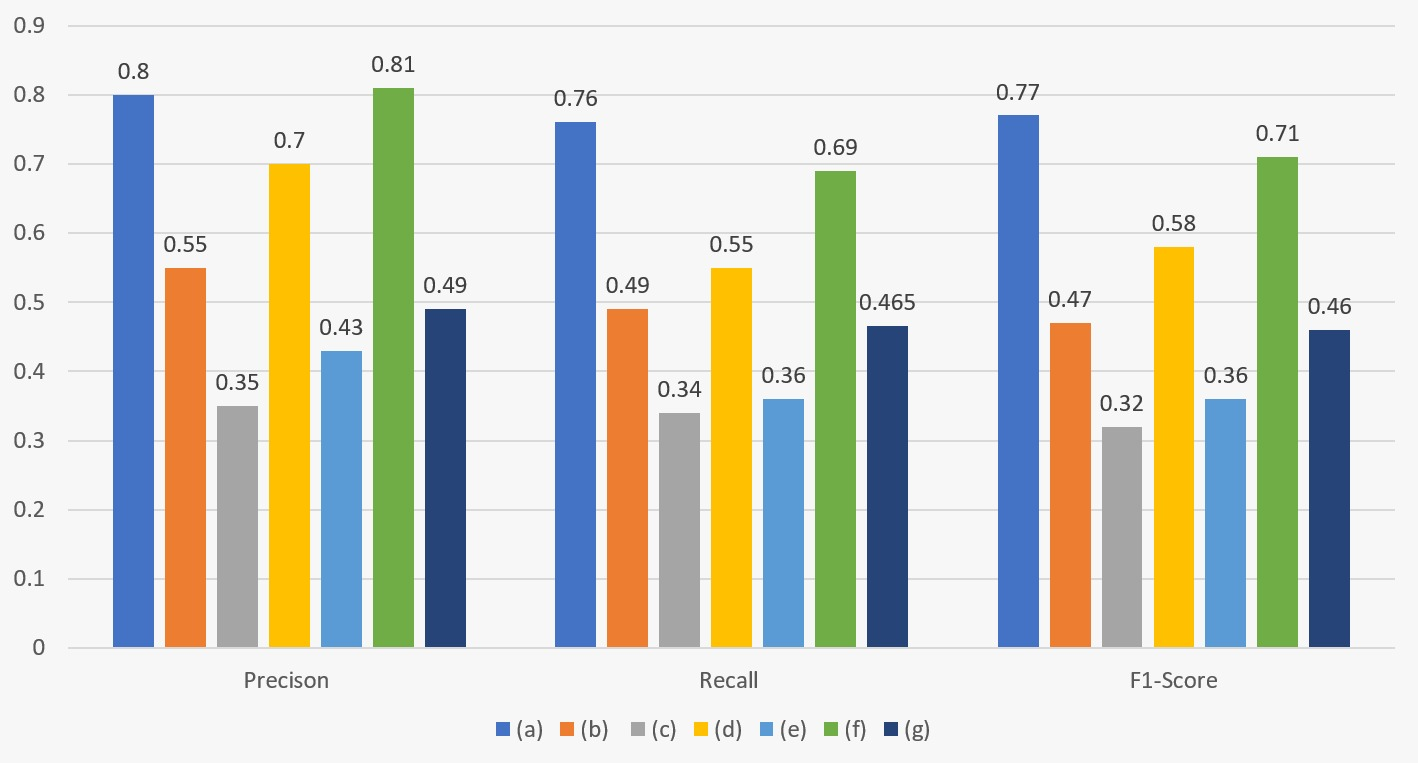
\includegraphics[width=15cm, keepaspectratio]{pics/Q1.jpeg}
    \caption{Macro-averaged \textit{Precision}, \textit{Recall} and \textit{F1-Score} of (a) Support Vector Machine trained on English corpus and evaluated on document level, (b) Bidirectional LSTM trained on English corpus without clustered data evaluated on document level, (c) Bidirectional LSTM trained on English corpus without clustered data, evaluated on sentence level, (d) Bidirectional LSTM trained on English and German corpus without clustered data, evaluated on document level, (e)
    Bidirectional LSTM trained on English and German corpus without clustered data, evaluated on sentence level, (f)
    Bidirectional LSTM on trained English and German corpus with clustered data, evaluated on document level, macro-average value is the average of macro-average values from cluster 1 and cluster 2  (g) Bidirectional LSTM trained on English and German corpus with clustered data, evaluated on sentence level, macro-average value is the average of macro-average values from cluster 1 and cluster 2. The performance evaluation of the clustered data is without the effect of the root classifier which classifies it into one of the two groups.}
    \label{fig:question1Eval}
\end{figure}

\ref{fig:question1Eval} (a) and (b) shows that the performance of the SVM is far more superior then Bidirectional LSTM when trained only on English corpus on document level. The result of the same Bidirectional LSTM when evaluated on sentence level is less compared to when evaluated on document level as illustrated in \ref{fig:question1Eval} (b) and (c). The results on the sentence level are significantly lower compared to the results on the document level. This behaviour can be further explained by considering an example document which is categorised in class $A$ and contains three sentences. As described in the \ref{backgroundSlidingWindow} all the three sentences of this document will have the same class as the document.
\begin{table}[!ht]
\centering
\begin{tabular}{>{\centering\arraybackslash}m{3cm}>{\centering\arraybackslash}m{3cm}>{\centering\arraybackslash}m{3cm}>{\centering\arraybackslash}m{3cm}}
\hline
\textbf{Sentence Identifier} & \textbf{Prediction Score of each class, [Class A, Class B]} & \textbf{True class} & \textbf{Predicted class} \\ \hline
Sentence I & {[}0.9, 0.1 {]} & A & A \\[0.2cm]
Sentence II & {[}0.49, 0.51{]} & A & B \\[0.2cm]
Sentence III & {[}0.45, 0.55{]} & A & B \\ [0.2cm]\hline
Summation of prediction score for the whole document (normalized) & {[}0.62 , 0.38{]} & A & A
\end{tabular}
\caption{Document with three sentences, prediction score for each class, true class and predicted class}
\label{table:SentVsDoc}
\end{table}

From the \ref{table:SentVsDoc}, we can see that the predicted score of \textit{Sentence I} for class $A$ is 0.9 and for class $B$ is 0.1, hence it is predicted in class A  but for \textit{Sentence B} and \textit{sentence C} although they belong to class $A$ they are predicted in class $B$ since the classifier was uncertain about the decision. However, when we combine the predicted score for all the classes from all the sentences and normalize them, the overall score for the document is higher for class $A$, so the precision of the above classifier on sentence level will be $\frac{1}{3} = 0.33$ and on document level the precision is $\frac{1}{1} = 1$ and therefore when evaluating on document level, the performance matrices will be better. 
\todo{Advantages of confidence values instead of heuristically assigning class label on the bases of majority vote.}


\ref{fig:question1Eval} (d) and (f) shows the effect of clustering. The specialization advantage of clustering improves the classification performance by approximately 10\% across \textit{precision, recall} and \textit{f1-score} on the document and approximately 7-10\% on the sentence level shown in \ref{fig:question1Eval} (e) and (g).

The \ref{tabel:LSTMCluster&NonClustered} shows the class-wise \textit{precision, recall} and \textit{F1-Score} values for Bidirectional LSTM trained on English and German corpus with clustering and without clustering.
\clearpage
\begin{table}[!ht]
\centering
\begin{tabular}{>{\raggedright\arraybackslash}m{5.8cm}>{\centering\arraybackslash}m{1cm}>{\centering\arraybackslash}m{1cm}>{\centering\arraybackslash}m{1cm}>{\centering\arraybackslash}m{1.1cm}>{\centering\arraybackslash}m{1.1cm}>{\centering\arraybackslash}m{1.1cm}}
\hline
Category & P$_\text{LSTM}$ &  R$_\text{LSTM}$ & F$_\text{LSTM}$ & P$_\text{LSTM-C}$ & R$_\text{LSTM-C}$ & F$_\text{LSTM-C}$ \\ \hline
Agriculture & 0.74 & 0.78 & 0.76 & {\ul 0.90} & \textbf{0.86} & \textit{0.88} \\
Audiovisual and Media & 0.00 & 0.00 & 0.00 & {\ul 1.00} & \textbf{0.10} & \textit{0.18} \\
Budget & {\ul 0.90} & 0.45 & 0.60 & 0.78 & \textbf{0.70} & \textit{0.74} \\
Competition & 0.90 & 0.63 & 0.75 & {\ul 0.96} & \textbf{0.83} & \textit{0.89} \\
Consumers & 0.54 & 0.54 & 0.54 & {\ul 0.59} & \textbf{0.65} & \textit{0.62} \\
Culture & 0.00 & 0.00 & 0.00 & {\ul 0.93} & \textbf{1.00} & \textit{0.97} \\
Customs & 0.78 & 0.47 & 0.58 & {\ul 0.64} & \textbf{0.70} & \textit{0.67} \\
Development & 0.45 & 0.81 & 0.57 & {\ul 0.64} & \textbf{0.83} & \textit{0.72} \\
Economic and Monetary Affairs & 0.85 & \textbf{0.93} & 0.89 & {\ul 0.95} & 0.87 & \textit{0.91} \\
Education Training Youth & 0.64 & 0.94 & 0.77 & {\ul 0.86} & 0.94 & \textit{0.90} \\
Employment and Social Policy & 0.68 & 0.83 & 0.75 & {\ul 0.71} & \textbf{0.88} & \textit{0.79} \\
Energy & 0.71 & \textbf{0.71} & 0.71 & {\ul 0.97} & 0.64 & \textit{0.77} \\
Enlargement & 0.70 & 0.44 & 0.54 & {\ul 0.76} & \textbf{0.59} & \textit{0.67} \\
Enterprise & 0.44 & 0.15 & 0.23 & {\ul 0.65} & \textbf{0.42} & \textit{0.51} \\
Environment & 0.69 & 0.82 & 0.75 & {\ul 0.70} & \textbf{0.84} & \textit{0.76} \\
External Relations & {\ul 1.00} & 0.23 & 0.37 & 0.92 & \textbf{0.55} & \textit{0.69} \\
External Trade & 0.53 & 0.61 & 0.57 & {\ul 0.61} & \textbf{0.71} & \textit{0.66} \\
Fight Against Fraud & {\ul 1.00} & 0.25 & 0.40 & 0.53 & \textbf{0.50} & \textit{0.52} \\
Food Safety & 0.90 & 0.82 & 0.86 & {\ul 0.93} & 0.82 & \textit{0.87} \\
Foreign and Security Policy & 0.65 & 0.54 & 0.59 & {\ul 0.62} & \textbf{0.83} & \textit{0.71} \\
Human Rights & 1.00 & 0.12 & 0.22 & {\ul 0.59} & \textbf{0.71} & \textit{0.64} \\
Humanitarian Aid & 1.00 & 0.29 & 0.44 & {\ul 0.67} & \textbf{0.57} & \textit{0.62} \\
Information Society & 0.54 & 0.72 & 0.62 & {\ul 0.71} & \textbf{0.84} & \textit{0.77} \\
Institutional Affairs & 0.62 & 0.60 & 0.61 & {\ul 0.67} & \textbf{0.65} & \textit{0.66} \\
Internal Market & 0.62 & 0.70 & 0.66 & {\ul 0.72} & \textbf{0.75} & \textit{0.74} \\
Justice Freedom Security & 0.53 & \textbf{0.86} & 0.66 & {\ul 0.81} & 0.67 & \textit{0.74} \\
Maritime Affairs and Fisheries & 0.91 & 0.80 & 0.85 & {\ul 0.94} & \textbf{0.91} & \textit{0.92} \\
Public Health & 1.00 & 0.39 & 0.56 & {\ul 0.86} & \textbf{0.43} & \textit{0.58} \\
Regional Policy & {\ul 0.88} & 0.50 & 0.64 & 0.72 & \textbf{0.86} & \textit{0.78} \\
Research Innovation & 0.71 & 0.43 & 0.53 & {\ul 0.60} & \textbf{0.96} & \textit{0.74} \\
Taxation & 0.94 & 0.54 & 0.68 & {\ul 0.95} & \textbf{0.71} & \textit{0.82} \\
Transport & 0.67 & 0.81 & 0.73 & {\ul 0.76} & \textbf{0.86} & \textit{0.81} \\ \hline

\end{tabular}
\caption{ Class-wise precision (P) and recall (R) and F1-Score (F) for the Bidirectional LSTM (denoted as LSTM for readability) trained on English and German corpus evaluated on document level. The suffix C indicates the results for clustered data. The best precision score among both the classifier is UNDERLINED, the best recall values among both the classifiers is in \textbf{bold} and the best F1-Score among both the classifiers is in \textit{italics}. 
}
\label{tabel:LSTMCluster&NonClustered}
\end{table}


It is evident from the \ref{tabel:LSTMCluster&NonClustered} that clustering indeed improves the performance of the classifiers. For the \textit{Audiovisual and Media} and \textit{Culture} classes we had less data, hence they were underrepresented for the first classifier with no clustering, but in the second classifier as the number of classes that needs to be predicted is less compared to the first cluster, these classes are predicted better than the first classifier.


\clearpage


\subsection{Evaluation for the second question}

In the second question the effects of general purpose resources such as word embeddings for the classification of legal domain specific task. All the classification models will be trained on English and German Corpora with clustering. 

The \ref{fig:SecondEvalQuestion} show the performance of different classifiers evaluated on sentence and document level.

\begin{figure}[!ht]
    \centering
    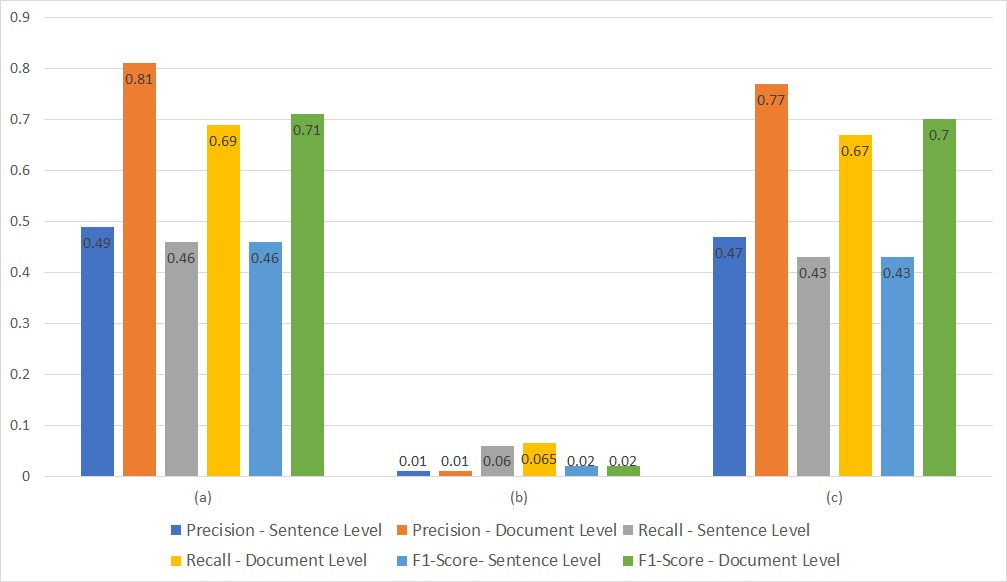
\includegraphics[width=15cm, keepaspectratio]{pics/FBMUSEQ2.jpg}
    \caption{Macro-average \textit{Precision}, \textit{Recall} and \textit{F1-Score} of (a) Bidirectional LSTM trained on English and German corpus with frozen domain specific word embeddings on clustered data and evaluated on document and sentence level, (b)  Bidirectional LSTM trained on English and German corpus, with frozen general purpose word embeddings (Facebook's MUSE) on clustered data and evaluated on both sentence and document level, (c) Bidirectional LSTM trained on English and German corpus, with trainable general purpose word embeddings (Facebook's MUSE) on clustered data and evaluated on both sentence and document level.}
    \label{fig:SecondEvalQuestion}
\end{figure}

From the \ref{fig:SecondEvalQuestion} it is quite evident that domain specific word embeddings perform notably better than the general purpose word embeddings. \ref{fig:SecondEvalQuestion} (a) shows the results of a classification model Bidirectional LSTM trained on English and German corpus with frozen domain specific word embeddings. Frozen word embedding here means that the embedding layer's weights will not be updated during the training of the network. \ref{fig:SecondEvalQuestion} (b) shows the results of a classification model Bidirectional LSTM trained on English and German corpus with frozen general purpose word embeddings, similar to the previous model, the weights of this model will not be updated. \ref{fig:SecondEvalQuestion} (c) shows the results of classification model Bidirectional LSTM trained on English and German corpus with trainable general purpose word embeddings, unlike the previous two models, in this model we are going to allow the model to update the weights of the embeddings. This was necessary to evaluate as the general purpose embeddings are trained on text from sources like Wikipedia or news article, which are not as complex in style and structure compared to legal text. This is the reason as to why it outperformed the model whose embedding weights were frozen. 

The classification model shown in \ref{fig:SecondEvalQuestion} (b) performed worst. It overfitted on the data and did predict everything to a single class. One of the reasons for this performance could be that the embedding matrix was never updated. As mentioned above that the general purpose word embeddings uses free text corpus such as Wikipedia and News articles, which contains information about multiple domains. Hence, when these embeddings were trained on Wikipedia and the News article corpus, the semantics captured is different from the one that is specifically trained on the legal corpus. One example of this can be seen in Image Recognition task when applying transfer learning; it is advisable that the dataset for prediction or classification task being performed should be similar to the ones we are doing transfer learning from \cite{iglovikov2018ternausnet}.


The results of \ref{fig:SecondEvalQuestion} (a) and (c) are comparable. The \ref{table:Evaal2} shows in detail the class-wise precision, recall and f1-score of Bidirectional LSTM trained on English and German corpus with the general purpose word embeddings and on the domain-specific word embeddings

% Please add the following required packages to your document preamble:
% \usepackage[normalem]{ulem}
% \useunder{\uline}{\ul}{}
\begin{table}[!ht]
\centering
\begin{tabular}{>{\raggedright\arraybackslash}m{5.8cm}>{\centering\arraybackslash}m{1cm}>{\centering\arraybackslash}m{1cm}>{\centering\arraybackslash}m{1cm}>{\centering\arraybackslash}m{1cm}>{\centering\arraybackslash}m{1cm}>{\centering\arraybackslash}m{1cm}}
\hline
Category & {\small P$_\text{\tiny {LSTM-D}}$} &  {\small R$_\text{{\tiny LSTM-D}}$} & {\small F$_\text{{\tiny LSTM-D}}$} & {\small P$_\text{{\tiny LSTM-G}}$} & {\small R$_\text{{\tiny LSTM-G}}$} & {\small F$_\text{{\tiny LSTM-G}}$} \\ \hline
Agriculture & {\ul 0.91} & \textbf{0.84} & \textit{0.87} & 0.82 & 0.80 & 0.81 \\
Audiovisual and Media & {\ul 1.00} & \textbf{0.30} & \textit{0.46} & 0.00 & 0.00 & 0.00 \\
Budget & {\ul 0.90} & \textbf{0.45} & \textit{0.60} & 0.67 & 0.20 & 0.31 \\
Competition & {\ul 0.93} & 0.83 & \textit{0.88} & 0.89 & 0.83 & 0.86 \\
Consumers & 0.62 & 0.61 & 0.62 & {\ul 0.65} & \textbf{0.65} & \textit{0.65} \\
Culture & 0.00 & 0.00 & 0.00 & {\ul 1.00} & \textbf{0.50} & \textit{0.67} \\
Customs & 0.87 & 0.43 & 0.58 & {\ul 0.94} & \textbf{0.53} & \textit{0.68} \\
Development & 0.42 & 0.81 & 0.55 & {\ul 0.64} & 0.81 & \textit{0.72} \\
Economic and Monetary Affairs & 0.85 & \textbf{0.99} & 0.91 & {\ul 0.90} & 0.95 & \textit{0.93} \\
Education Training Youth & 0.63 & 0.94 & 0.75 & {\ul 0.91} & 0.94 & \textit{0.92} \\
Employment and Social Policy & {\ul 0.77} & \textbf{0.87} & \textit{0.82} & 0.71 & 0.86 & 0.78 \\
Energy & {\ul 1.00} & \textbf{0.75} & \textit{0.86} & 0.98 & 0.71 & 0.82 \\
Enlargement & {\ul 0.70} & \textbf{0.66} & \textit{0.68} & 0.65 & 0.62 & 0.63 \\
Enterprise & {\ul 0.67} & \textbf{0.46} & \textit{0.55} & 0.64 & 0.35 & 0.45 \\
Environment & 0.75 & 0.88 & 0.81 & {\ul 0.80} & \textbf{0.89} & \textit{0.84} \\
External Relations & {\ul 1.00} & 0.05 & 0.09 & 0.68 & \textbf{0.59} & \textit{0.63} \\
External Trade & 0.55 & \textbf{0.64} & \textit{0.59} & {\ul 0.72} & 0.46 & 0.57 \\
Fight Against Fraud & {\ul 1.00} & 0.25 & 0.40 & 0.83 & \textbf{0.31} & \textit{0.45} \\
Food Safety & {\ul 0.90} & 0.80 & 0.85 & 0.84 & \textbf{0.87} & 0.85 \\
Foreign and Security Policy & 0.62 & 0.54 & 0.58 & {\ul 0.79} & \textbf{0.62} & \textit{0.70} \\
Human Rights & 0.83 & 0.21 & 0.33 & {\ul 0.89} & \textbf{0.33} & \textit{0.48} \\
Humanitarian Aid & 0.86 & 0.43 & 0.57 & {\ul 1.00} & \textbf{0.57} & \textit{0.73} \\
Information Society & 0.72 & 0.85 & 0.78 & {\ul 0.76} & \textbf{0.90} & \textit{0.82} \\
Institutional Affairs & {\ul 0.67} & 0.65 & \textit{0.66} & 0.55 & \textbf{0.80} & 0.65 \\
Internal Market & 0.71 & \textbf{0.81} & 0.75 & {\ul 0.74} & 0.80 & \textit{0.77} \\
Justice Freedom Security & 0.64 & \textbf{0.91} & 0.75 & {\ul 0.69} & 0.89 & \textit{0.78} \\
Maritime Affairs and Fisheries & {\ul 0.92} & \textbf{0.91} & \textit{0.92} & 0.87 & 0.89 & 0.88 \\
Public Health & 0.89 & \textbf{0.55} & \textit{0.68} & {\ul 0.92} & 0.52 & 0.67 \\
Regional Policy & {\ul 0.88} & 0.67 & 0.76 & 0.81 & \textbf{0.90} & \textit{0.85} \\
Research Innovation & 0.73 & 0.79 & 0.76 & {\ul 0.79} & 0.79 & \textit{0.79} \\
Taxation & 0.95 & \textbf{0.71} & \textit{0.82} & 0.95 & 0.64 & 0.77 \\
Transport & 0.79 & 0.84 & 0.81 & {\ul 0.82} & \textbf{0.89} & \textit{0.85} \\ \hline
\end{tabular}
\caption{My caption}
\label{table:Evaal2}
\end{table}


\subsection{Evaluation for third research question}

The third research question investigates the effect of having a multilingual parallel corpus on the classification task. A multilingual parallel corpus here means having different language documents for a predefined category. 

As described in \ref{fig:FlowResearchQuestion2} two Bidirectional LSTM classification models, one trained with English corpus and other trained with German corpus are compared with a single Bidirectional LSTM classification model trained on English and German corpus.

\begin{figure}[!ht]
    \centering
    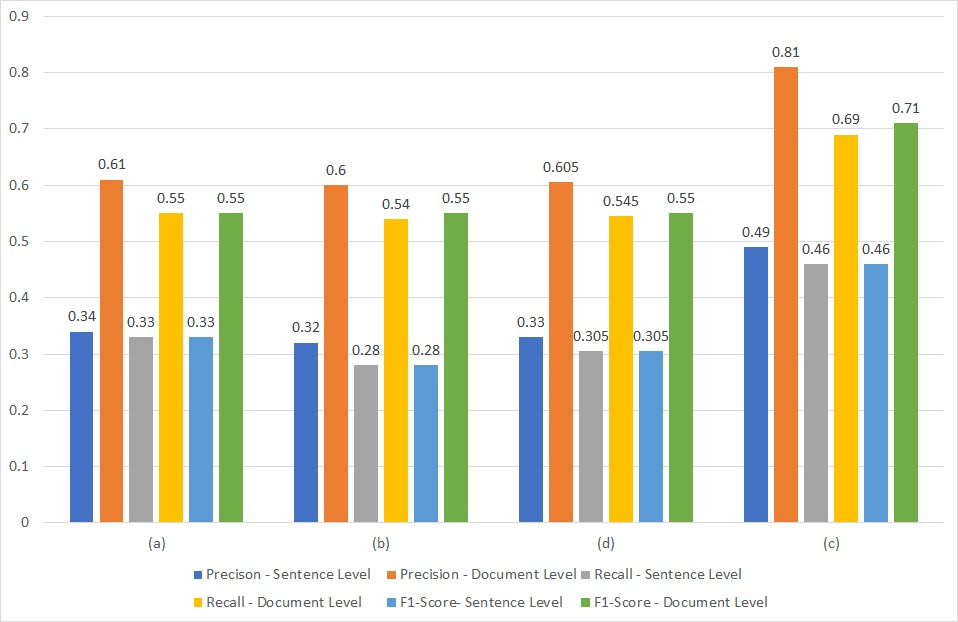
\includegraphics[width=15cm, keepaspectratio]{pics/Q3.jpg}
    \caption{Caption}
    \label{fig:EvaluationQuestion3}
\end{figure}

\ref{fig:EvaluationQuestion3} (a) and (b) shows that employing a single classifier for bilingual corpus is considerably better than two different classifiers for two different languages. 
One explanation for the better performance of the bilingual classifier is that it has more example to learn from than the previous case. C.-P. Wei et al. showed that polylingual data can be used to increase the performance of a classifier \cite{Wei:2014:EPD:2566999.2567111}. Also the clustering of the data would have helped as compared to unclustered data as shown in \ref{tabel:LSTMCluster&NonClustered} and  \ref{fig:question1Eval}. Although it was evident that adding more languages would have helped in improving the classification performance of the classifier from \ref{EvalQ1}, but at that point we had no information about the performance of a classifier trained on other corpus namely, German. 
